\documentclass[]{article}
\usepackage{lmodern}
\usepackage{amssymb,amsmath}
\usepackage{ifxetex,ifluatex}
\usepackage{fixltx2e} % provides \textsubscript
\ifnum 0\ifxetex 1\fi\ifluatex 1\fi=0 % if pdftex
  \usepackage[T1]{fontenc}
  \usepackage[utf8]{inputenc}
\else % if luatex or xelatex
  \ifxetex
    \usepackage{mathspec}
  \else
    \usepackage{fontspec}
  \fi
  \defaultfontfeatures{Ligatures=TeX,Scale=MatchLowercase}
\fi
% use upquote if available, for straight quotes in verbatim environments
\IfFileExists{upquote.sty}{\usepackage{upquote}}{}
% use microtype if available
\IfFileExists{microtype.sty}{%
\usepackage{microtype}
\UseMicrotypeSet[protrusion]{basicmath} % disable protrusion for tt fonts
}{}
\usepackage[margin=1in]{geometry}
\usepackage{hyperref}
\hypersetup{unicode=true,
            pdftitle={Estatística Básica},
            pdfauthor={Luan Fiorentin},
            pdfborder={0 0 0},
            breaklinks=true}
\urlstyle{same}  % don't use monospace font for urls
\usepackage{graphicx,grffile}
\makeatletter
\def\maxwidth{\ifdim\Gin@nat@width>\linewidth\linewidth\else\Gin@nat@width\fi}
\def\maxheight{\ifdim\Gin@nat@height>\textheight\textheight\else\Gin@nat@height\fi}
\makeatother
% Scale images if necessary, so that they will not overflow the page
% margins by default, and it is still possible to overwrite the defaults
% using explicit options in \includegraphics[width, height, ...]{}
\setkeys{Gin}{width=\maxwidth,height=\maxheight,keepaspectratio}
\IfFileExists{parskip.sty}{%
\usepackage{parskip}
}{% else
\setlength{\parindent}{0pt}
\setlength{\parskip}{6pt plus 2pt minus 1pt}
}
\setlength{\emergencystretch}{3em}  % prevent overfull lines
\providecommand{\tightlist}{%
  \setlength{\itemsep}{0pt}\setlength{\parskip}{0pt}}
\setcounter{secnumdepth}{0}
% Redefines (sub)paragraphs to behave more like sections
\ifx\paragraph\undefined\else
\let\oldparagraph\paragraph
\renewcommand{\paragraph}[1]{\oldparagraph{#1}\mbox{}}
\fi
\ifx\subparagraph\undefined\else
\let\oldsubparagraph\subparagraph
\renewcommand{\subparagraph}[1]{\oldsubparagraph{#1}\mbox{}}
\fi

%%% Use protect on footnotes to avoid problems with footnotes in titles
\let\rmarkdownfootnote\footnote%
\def\footnote{\protect\rmarkdownfootnote}

%%% Change title format to be more compact
\usepackage{titling}

% Create subtitle command for use in maketitle
\newcommand{\subtitle}[1]{
  \posttitle{
    \begin{center}\large#1\end{center}
    }
}

\setlength{\droptitle}{-2em}

  \title{Estatística Básica}
    \pretitle{\vspace{\droptitle}\centering\huge}
  \posttitle{\par}
  \subtitle{Lista 2 - Medidas Resumo}
  \author{Luan Fiorentin}
    \preauthor{\centering\large\emph}
  \postauthor{\par}
      \predate{\centering\large\emph}
  \postdate{\par}
    \date{2019-03-05}

\usepackage{amsmath} \usepackage{float} \usepackage{bm}

\begin{document}
\maketitle

\begin{enumerate}
\def\labelenumi{\arabic{enumi}.}
\tightlist
\item
  Um exame de vestibular para uma faculdade tem 80 questões, sendo 40 de
  português e 40 de matemática. Para os 20 melhores classificados,
  apresentamos o número de acertos em cada disciplina, com os valores já
  ordenados.

  \begin{itemize}
  \tightlist
  \item
    Português: (8; 10; 11; 12; 12; 14; 17; 20; 20; 23; 23; 24; 26; 26;
    30; 31; 32; 34; 35; 35)
  \item
    Matemática: (13; 20; 20; 20; 21; 21; 23; 23; 25; 25; 26; 27; 28; 28;
    28; 29; 30; 31; 31; 32)
  \end{itemize}

  \begin{enumerate}
  \def\labelenumii{(\alph{enumii})}
  \tightlist
  \item
    Calcule as medidas de centro (média, mediana e moda) para cada
    grupo.
  \item
    Calcule as medidas de variabilidade (variância, desvio-padrão, e
    coeficiente de variação) para cada grupo.
  \item
    Calcule os quartis para cada grupo.
  \item
    Construa um gráfico de caixa (box plot) para cada grupo (em um mesmo
    gráfico para comparação).
  \item
    Com todos os resultados obtidos, descreva comparativamente os dois
    grupos em termos de medidas de tendência central, variabilidade,
    amplitude e distribuição (simetria) dos dados.
  \item
    Você acha que os aprovados são melhores em português ou matemática?
  \end{enumerate}
\item
  Considere a amostras de alturas de uma espécie de árvore (metros),
  coletadas em quatro áreas diferentes.

  \begin{itemize}
  \tightlist
  \item
    Área A: (9,2; 10,8; 10,6; 11,1; 12,1; 9,6; 11,2; 8,4; 12,9; 12,1;
    14,4; 11,1; 11,1; 9,7; 8,4; 12,3; 10,7; 12,9; 9,1; 12,8).
  \item
    Área B: (12,5; 18,5; 21,3; 14,3; 18,5; 19,0; 10,8; 23,1; 17,4; 10,7;
    14,3; 16,3; 18,0; 7,1; 12,8; 14,7; 11,3; 8,2; 13,8).
  \item
    Área C: (21,3; 28,7; 15,8; 24,0; 13,7; 18,1; 12,6; 14,6; 6,1; 19,8;
    22,3; 15,7; 16,3; 18,2; 15,7; 6,6; 9,3; 1,3; 19,0).
  \item
    Área D: (13,7; 8,6; 14,9; 10,2; 14,0; 10,5; 15,0; 5,2; 10,0; 11,7;
    18,7; 9,3; 7,9; 6,5; 11,5; 12,0; 8,3; 8,3; 9,8; 4,7).
  \end{itemize}

  \begin{enumerate}
  \def\labelenumii{(\alph{enumii})}
  \tightlist
  \item
    Calcule as medidas de amplitude, média, mediana, variância, desvio
    padrão e coeficiente de variação para as quatro áreas.
  \item
    Descreva comparativamente as quatro áreas quanto à altura das
    árvores, utilizando as estatísticas que você calculou.
  \end{enumerate}
\item
  Deseja-se comparar três métodos de ensino no aprendizado de
  estatística. Cada método foi aplicado a 30 alunos e os resultados
  estão apresentados nos boxplot abaixo.

  \begin{enumerate}
  \def\labelenumii{(\alph{enumii})}
  \tightlist
  \item
    Encontre os valores (aproximados) para a mediana, os quartis, máximo
    e mínimo.
  \item
    Discuta a variabilidade do tempo de aprendizado de cada método.
  \item
    Se você é otimista, qual método escolheria?
  \end{enumerate}
\end{enumerate}

\begin{figure}[H]
\centering
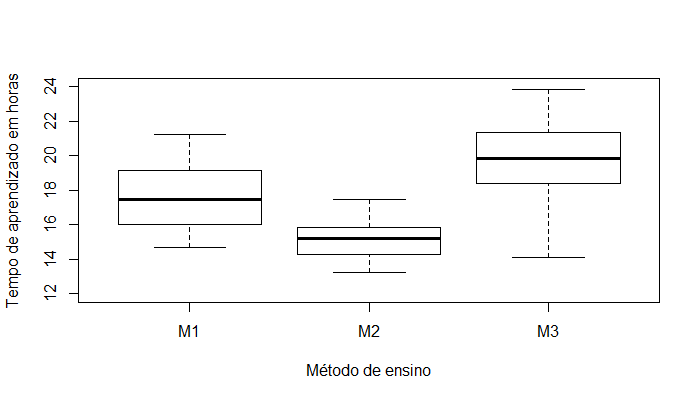
\includegraphics[]{ex3.PNG}
\end{figure}

\begin{enumerate}
\def\labelenumi{\arabic{enumi}.}
\setcounter{enumi}{3}
\tightlist
\item
  A distribuição das estaturas, em centímetros, de alunos de um curso
  colegial está representada na tabela de frequência abaixo. Calcule a
  média, a variância, e o desvio-padrão das estaturas.
\end{enumerate}

\begin{table}[H]
\centering
\begin{tabular}{cc}
\hline
Classes     & Frequência \\ \hline
{[}135-145) & 15         \\
{[}145-155) & 150        \\
{[}155-165) & 250        \\
{[}165-175) & 70         \\
{[}175-185) & 10         \\
{[}185-195] & 5          \\ \hline
\end{tabular}
\end{table}

\begin{enumerate}
\def\labelenumi{\arabic{enumi}.}
\setcounter{enumi}{4}
\tightlist
\item
  Os dados abaixo representam as vendas semanais, em classes de salários
  mínimos, de vendedores de gêneros alimentícios:

  \begin{enumerate}
  \def\labelenumii{(\alph{enumii})}
  \tightlist
  \item
    Faça o histograma das observações.
  \item
    Calcule a média da amostra (\(\bar x\)).
  \item
    Calcule o desvio-padrão da amostra.
  \item
    Calcule o primeiro quartil (\(Q_1\)), mediana (\(Q_2\)) e o terceiro
    quartil (\(Q_3\)).
  \end{enumerate}
\end{enumerate}

\begin{table}[H]
\centering
\begin{tabular}{cc}
\hline
Vendas    & Vendedores \\ \hline
{[}30-35) & 2          \\
{[}35-40) & 10         \\
{[}40-45) & 18         \\
{[}45-50) & 50         \\
{[}50-55) & 70         \\
{[}55-60) & 30         \\
{[}60-65) & 18         \\
{[}65-70) & 2          \\ \hline
\end{tabular}
\end{table}

\begin{enumerate}
\def\labelenumi{\arabic{enumi}.}
\setcounter{enumi}{5}
\tightlist
\item
  O departamento pessoal de uma certa firma fez um levantamento dos
  salários dos 120 funcionários do setor administrativo, obtendo os
  resultados (em salários mínimos) da tabela abaixo.

  \begin{enumerate}
  \def\labelenumii{(\alph{enumii})}
  \tightlist
  \item
    Calcule a média, a mediana, a variância e o desvio-padrão
  \item
    Se for concedido um aumento de 100\% para todos os 120 funcionários,
    haverá alteração na média? E na variância? Justifique sua resposta.
  \item
    Se for concedido um abono de dois salários mínimos para todos os 120
    funcionários, haverá alteração na média? E na mediana? E na
    variância? Justifique sua resposta.
  \end{enumerate}
\end{enumerate}

\begin{table}[H]
\centering
\begin{tabular}{ll}
\hline
Salários   & Freq. relativa \\ \hline
{[}0-2)    & 0,25           \\
{[}2-4)    & 0,40           \\
{[}4-6)    & 0,20           \\
{[}6-10{]} & 0,15           \\ \hline
\end{tabular}
\end{table}

\begin{enumerate}
\def\labelenumi{\arabic{enumi}.}
\setcounter{enumi}{6}
\tightlist
\item
  O resultado de uma prova de estatística aplicada à 25 alunos foi o
  seguinte:
\end{enumerate}

\[(9, 9, 8, 8, 9, 10, 8, 8, 9, 8, 10, 7, 7, 9, 9, 7, 8, 9, 4, 7, 7, 8, 10, 9, 9)\]

Como os alunos possuiam diferentes níveis educacionais, decidiu-se
calcular o desempenho relativo de cada candidato, para facilitar a
interpretação dos resultados. Essa medida de desempenho relativo será
obtida da seguinte forma: 1. Calcula-se a média (\(\bar x\)) e o
desvio-padrão (\(s\)) da amostra. 2. A nota \(x_i\) de cada aluno será
padronizada da seguinte forma:

\[z_i = \frac{x_i - \bar x}{s}.\]

Assim, criou-se uma nova variável \(Z\) que corresponde ao conjunto de
notas padronizadas. Com isso:

\begin{enumerate}
\def\labelenumi{(\alph{enumi})}
\tightlist
\item
  Calcule as notas padronizadas de todos os funcionários.
\item
  Com os resultados obtidos acima, calcule a média (\(\bar z\)) e o
  desvio-padrão (\(s_z\)) de \(Z\).
\item
  Se alguma das notas padronizadas estiver acima de \(2s_z\) ou abaixo
  de \(-2s_z\), esse aluno deve ser considerado ``atípico''. Existe
  algum nessa situação?
\item
  Interprete o significado de \(Z\).
\end{enumerate}


\end{document}
